\documentclass[12pt,a4paper]{article}
\usepackage[utf8]{inputenc}
\usepackage{geometry}
\usepackage{titlesec} % For customizing section titles
\usepackage{graphicx} % For images
\usepackage{hyperref} % For hyperlinks
\usepackage{fancyhdr} % For fancy headers and footers
\usepackage{lipsum} % For generating dummy text
\usepackage{graphicx}
\usepackage{subcaption}
\usepackage{dirtree}
\usepackage{float}
% Set page geometry
\geometry{left=2.5cm, right=2.5cm, top=2.5cm, bottom=2.5cm}

% Set up hyperref
% Set up hyperref
\hypersetup{
    colorlinks=true,
    allcolors=blue,
    linkcolor=black,
    filecolor=cyan,
    urlcolor=blue,
}

% Customize section titles
\titleformat{\section}{\large\bfseries}{\thesection}{1em}{}
\titleformat{\subsection}{\normalsize\bfseries}{\thesubsection}{1em}{}

% Setup headers and footers
\pagestyle{fancy}
\fancyhf{}
\rhead{3D printing defect detection}
\lhead{Summarization}
\rfoot{Page \thepage}

% Title and author
\title{{\textbf{Summarization of AI project 3D printing defect}}}
\author{Michal Raczkowski}
\date{26-01-2024}

\begin{document}

\maketitle
\thispagestyle{empty} % Remove header/footer for the first page

% Insert table of contents
\newpage
\tableofcontents
\newpage

\setcounter{page}{1} % Start page numbering from here




\section{Objectives}
\begin{itemize}
    \item \textbf{Objective}: Identify "spaghetti" defects in 3D printed models.
    \item \textbf{Target Variable}: "Defect Status" (0 for absent, 1 for present).
\end{itemize}

\section{Goal}
\begin{itemize}
    \item \textbf{Goal}: Detect "spaghetti" defects at an early stage of 3D printing to halt the process, thereby conserving materials and electricity.
\end{itemize}

\section{Data Requirements}
\begin{itemize}
    \item \textbf{Type}: Images 
    \item \textbf{Color}: Black and White (Grayscale)
    \item \textbf{Format}: .jpeg, .png
    \item \textbf{Resolution}: min. 640x480 px
    \item \textbf{Content}: Displaying "spaghetti" defect with nozzle above and print on the 3d printer bed
    \item \textbf{Example}:
    \begin{figure}[h]
        \centering
        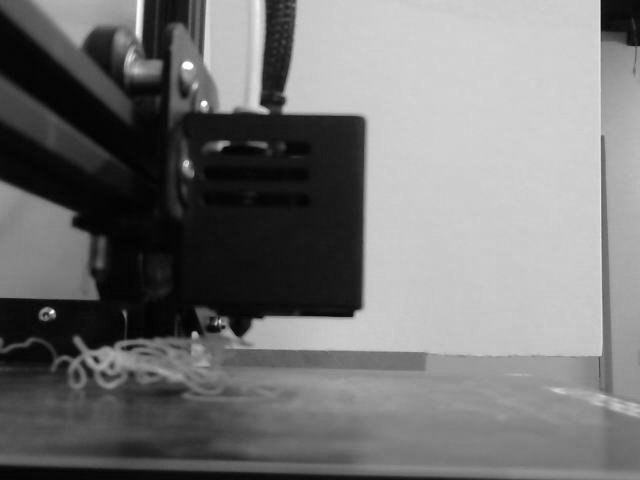
\includegraphics[width=0.5\linewidth]{no_support_57.jpg}
        \caption{Example picture \cite{onlineOpenSource1}}
        \label{fig:spaghetti3D}
    \end{figure}
        
\end{itemize}

\section{Data Sources}
\begin{itemize}
    \item Homemade pictures and open-source online repositories. {\scriptsize\cite{onlineOpenSource1}} {\scriptsize\cite{onlineOpenSource2}}
\end{itemize}

\section{Data Preparation}
\begin{itemize}
    \item Choose relevant (with "spaghetti" defect) images from datasets
    \item Change color to black and white (grayscale)
    \item Rotate some of them 
\end{itemize}

\section{Data Legality and Ethics}
\begin{itemize}
    \item Data legally obtained with rights of open source
\end{itemize}

\section{Data Diversity}
\begin{itemize}
    \item Marge images from online sources and homemade images, some images are rotated to increase amount of data and increase diversity
\end{itemize}

\section{Version Control}
\begin{itemize}
    \item GIT
\end{itemize}

\section{Used tools}
\begin{itemize}
    \item Computer Vision Annotation Tool: CVAT {\scriptsize\cite{labelingTool1}}
    \item Object Tagging Tool: VoTT {\scriptsize\cite{labelingTool2}}
    \item Labeling tool: MakeSense {\scriptsize\cite{labelingTool3}}
    \item Image processing tool: Resizepixel {\scriptsize\cite{imagesOnlineTool}} 
\end{itemize}

\section{Modeling}
\begin{itemize}
    \item \textbf{Approach}: Use YOLOv8 (CNN)
    \item \textbf{Metrics} IoU, AP, mAP, Precision, Recall, F1 Score.
\end{itemize}


\section{Code}
The absence of a notebook is not due to a lack of extensive code for training the model; rather, it's attributed to the nature of YOLOv8. Additionally, data manipulation was carried out using external tools, as this approach was more efficient.

Here is code: 
\begin{verbatim}
    from ultralytics import YOLO

    model = YOLO("yolov8n.yaml")  
    
    results = model.train(data="config.yaml", epochs=20) 
\end{verbatim}

\newpage

Here is configuration which is crucial for YOLOv8: 

\begin{verbatim}
    ath: /home/michal/Repos/OpenWeekProject/data # dataset root dir
    train: images/train # train images (relative to 'path')
    val: images/val # val images (relative to 'path')
    
    # Classes
    names:
      0: spaghetti
    
\end{verbatim}


\section{Results}


\begin{figure}[h]
    \centering
    \makebox[\textwidth][c]{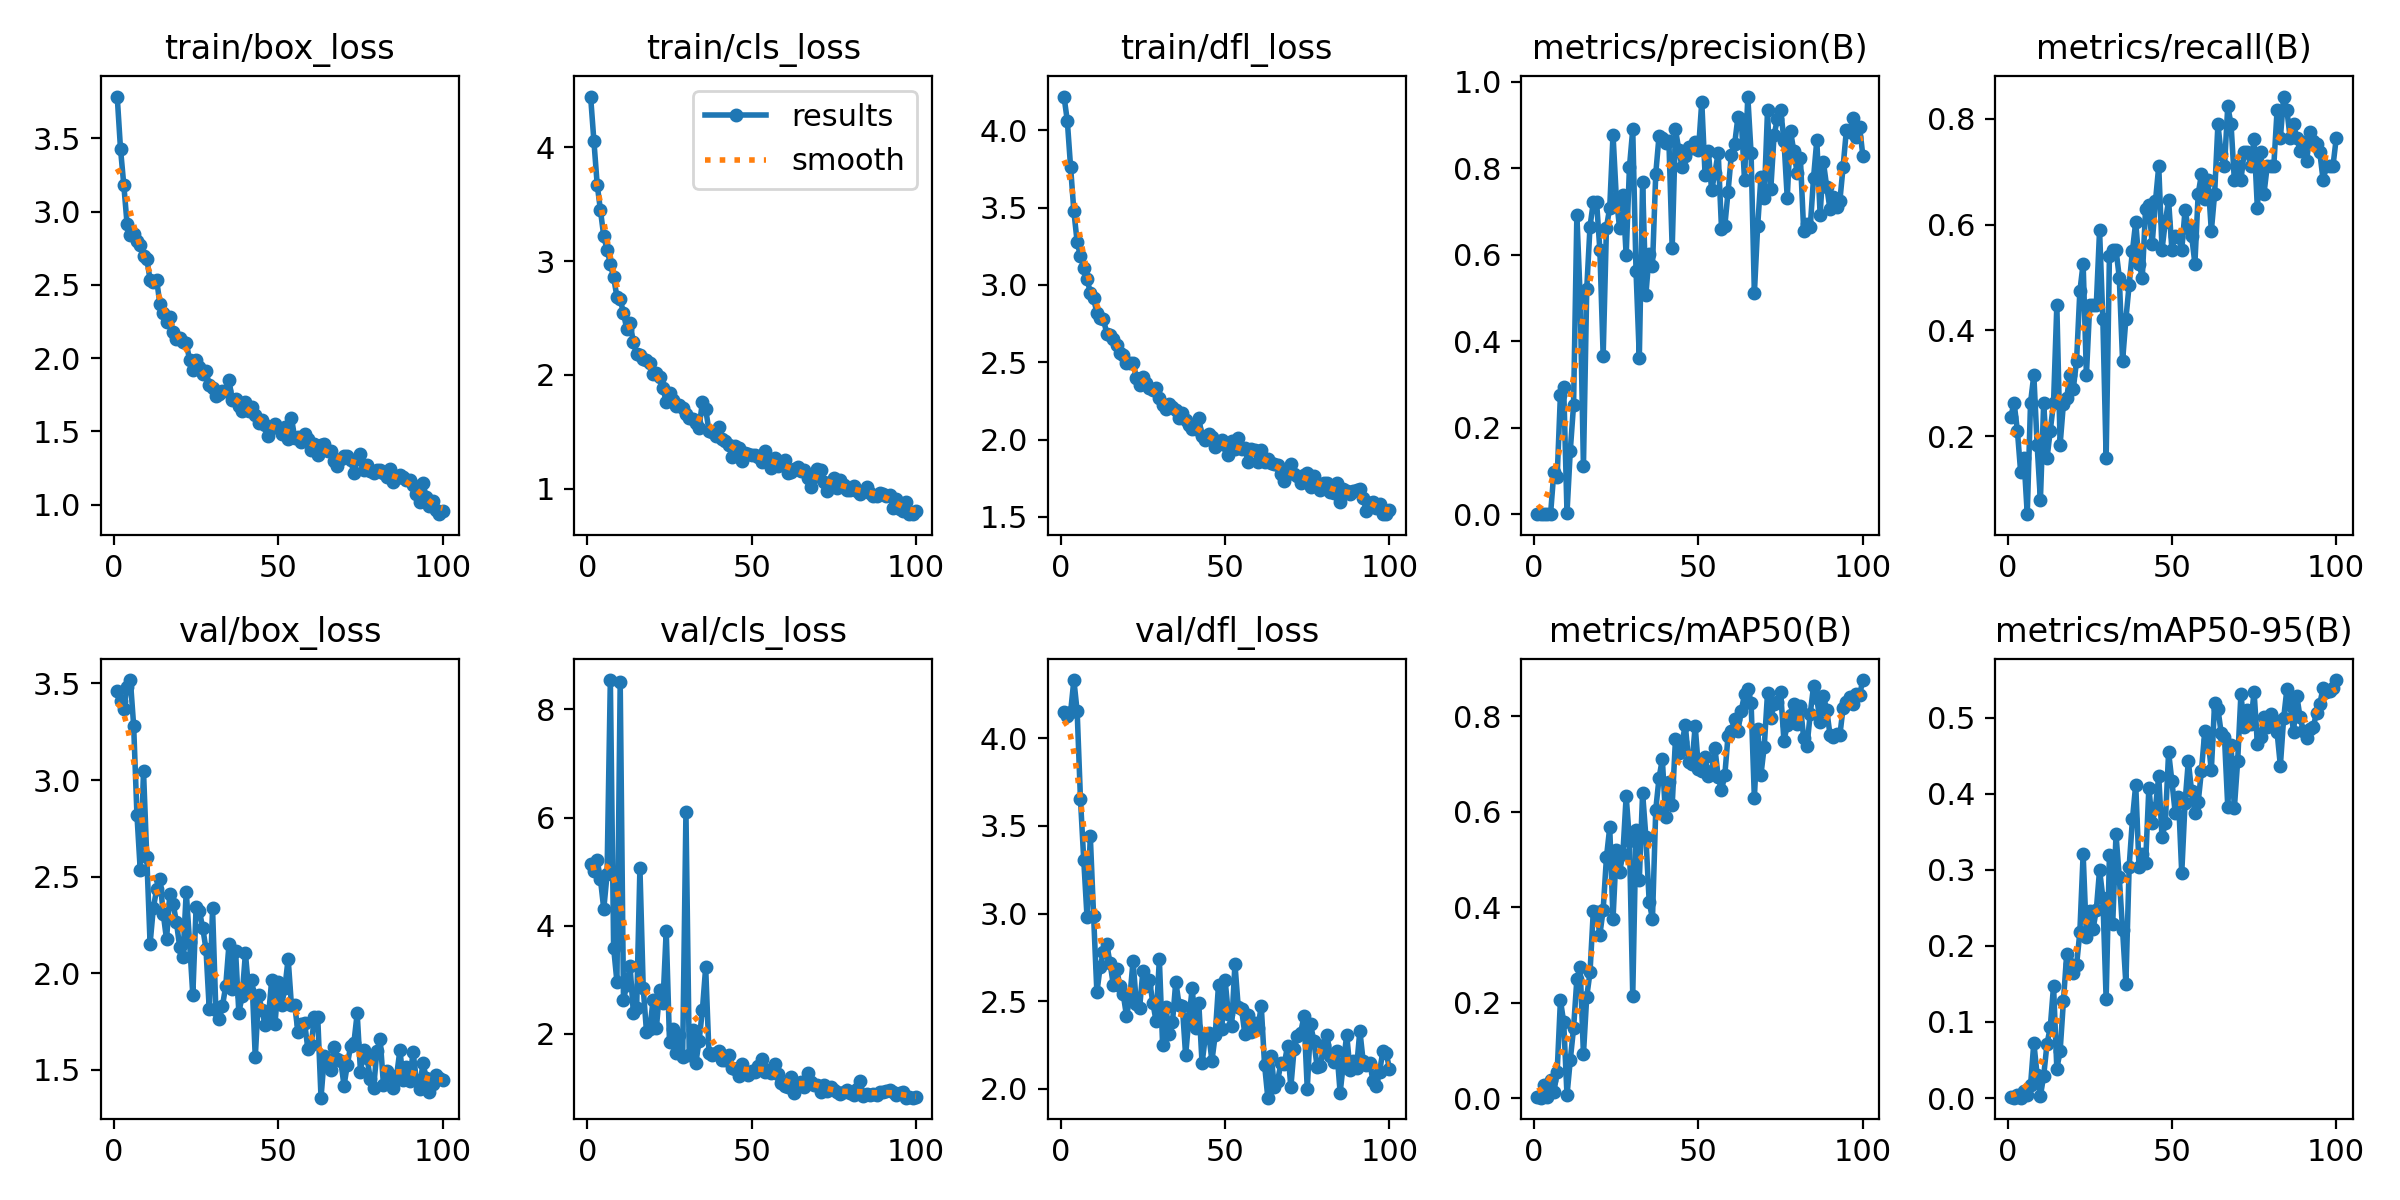
\includegraphics[width=1.2\linewidth]{results.png}}
    \caption{Graph Result}
    \label{fig:grpahresult}
\end{figure}

\begin{figure}[htp]
    \centering
    \makebox[\textwidth][c]{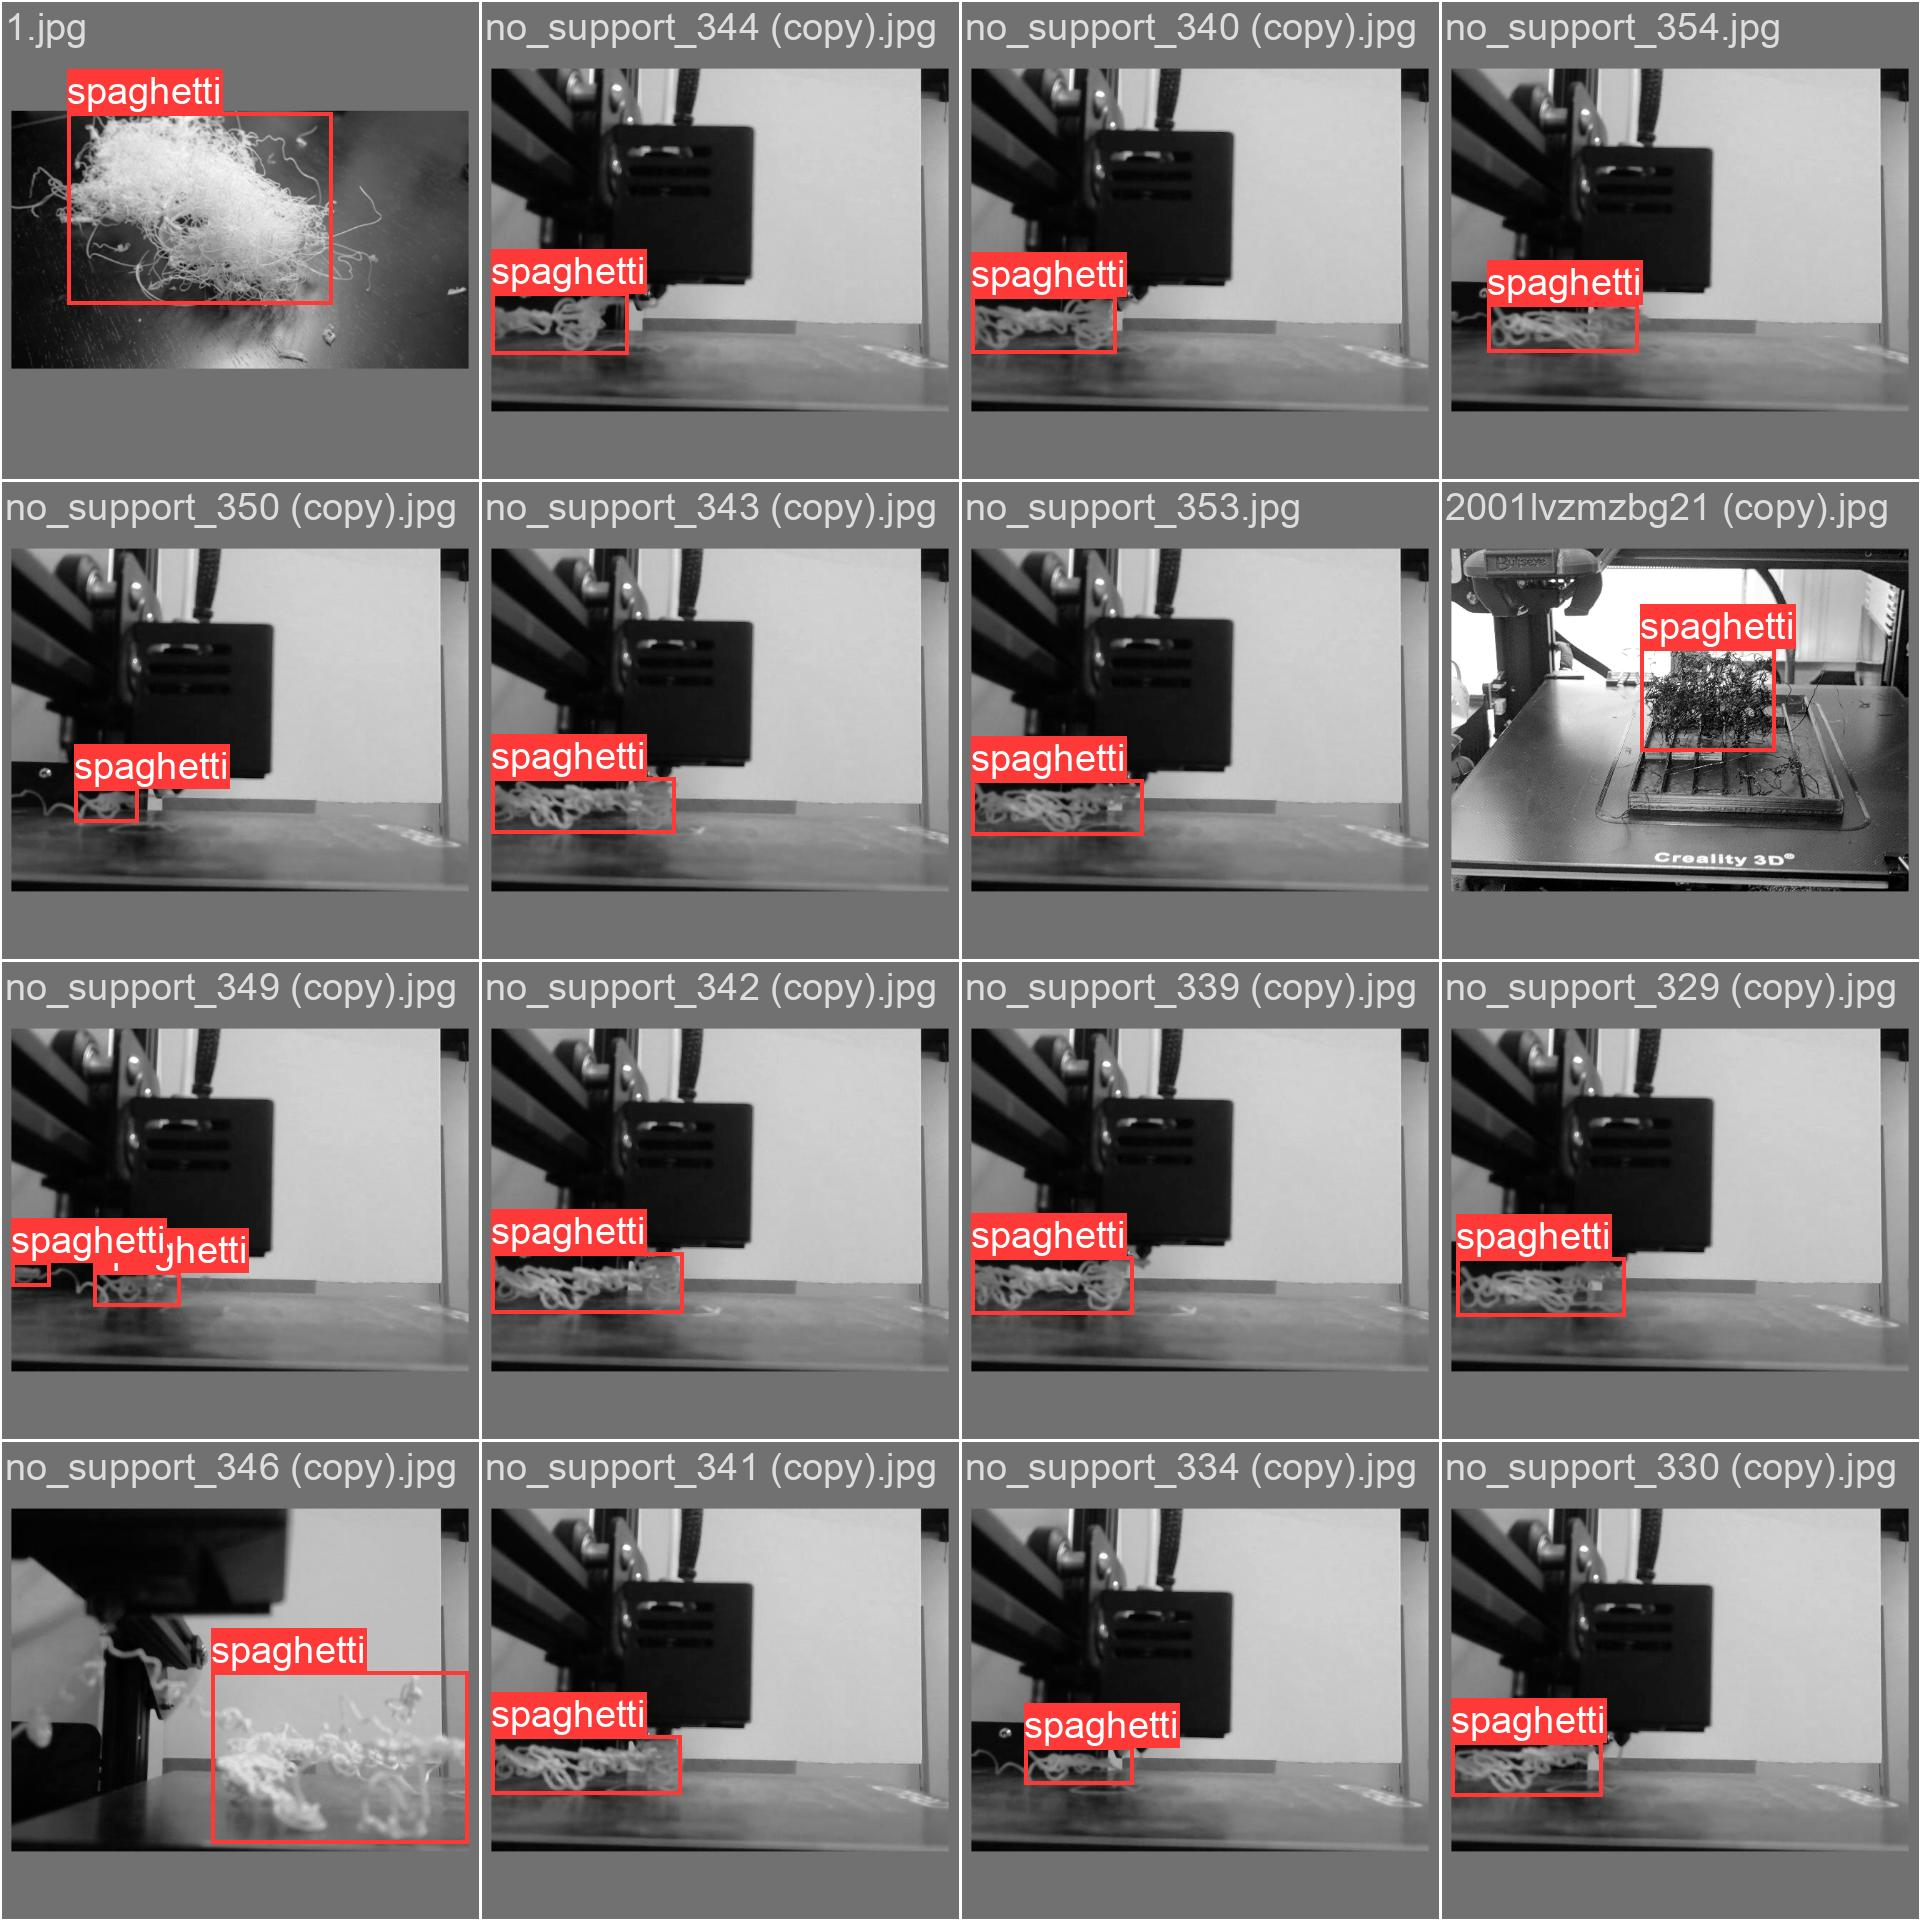
\includegraphics[width=1.2\linewidth]{val_batch0_labels.jpg}}
    \caption{Labels on Images}
    \label{fig:grpahLabels}
\end{figure}

\begin{figure}[h]
    \centering
    \makebox[\textwidth][c]{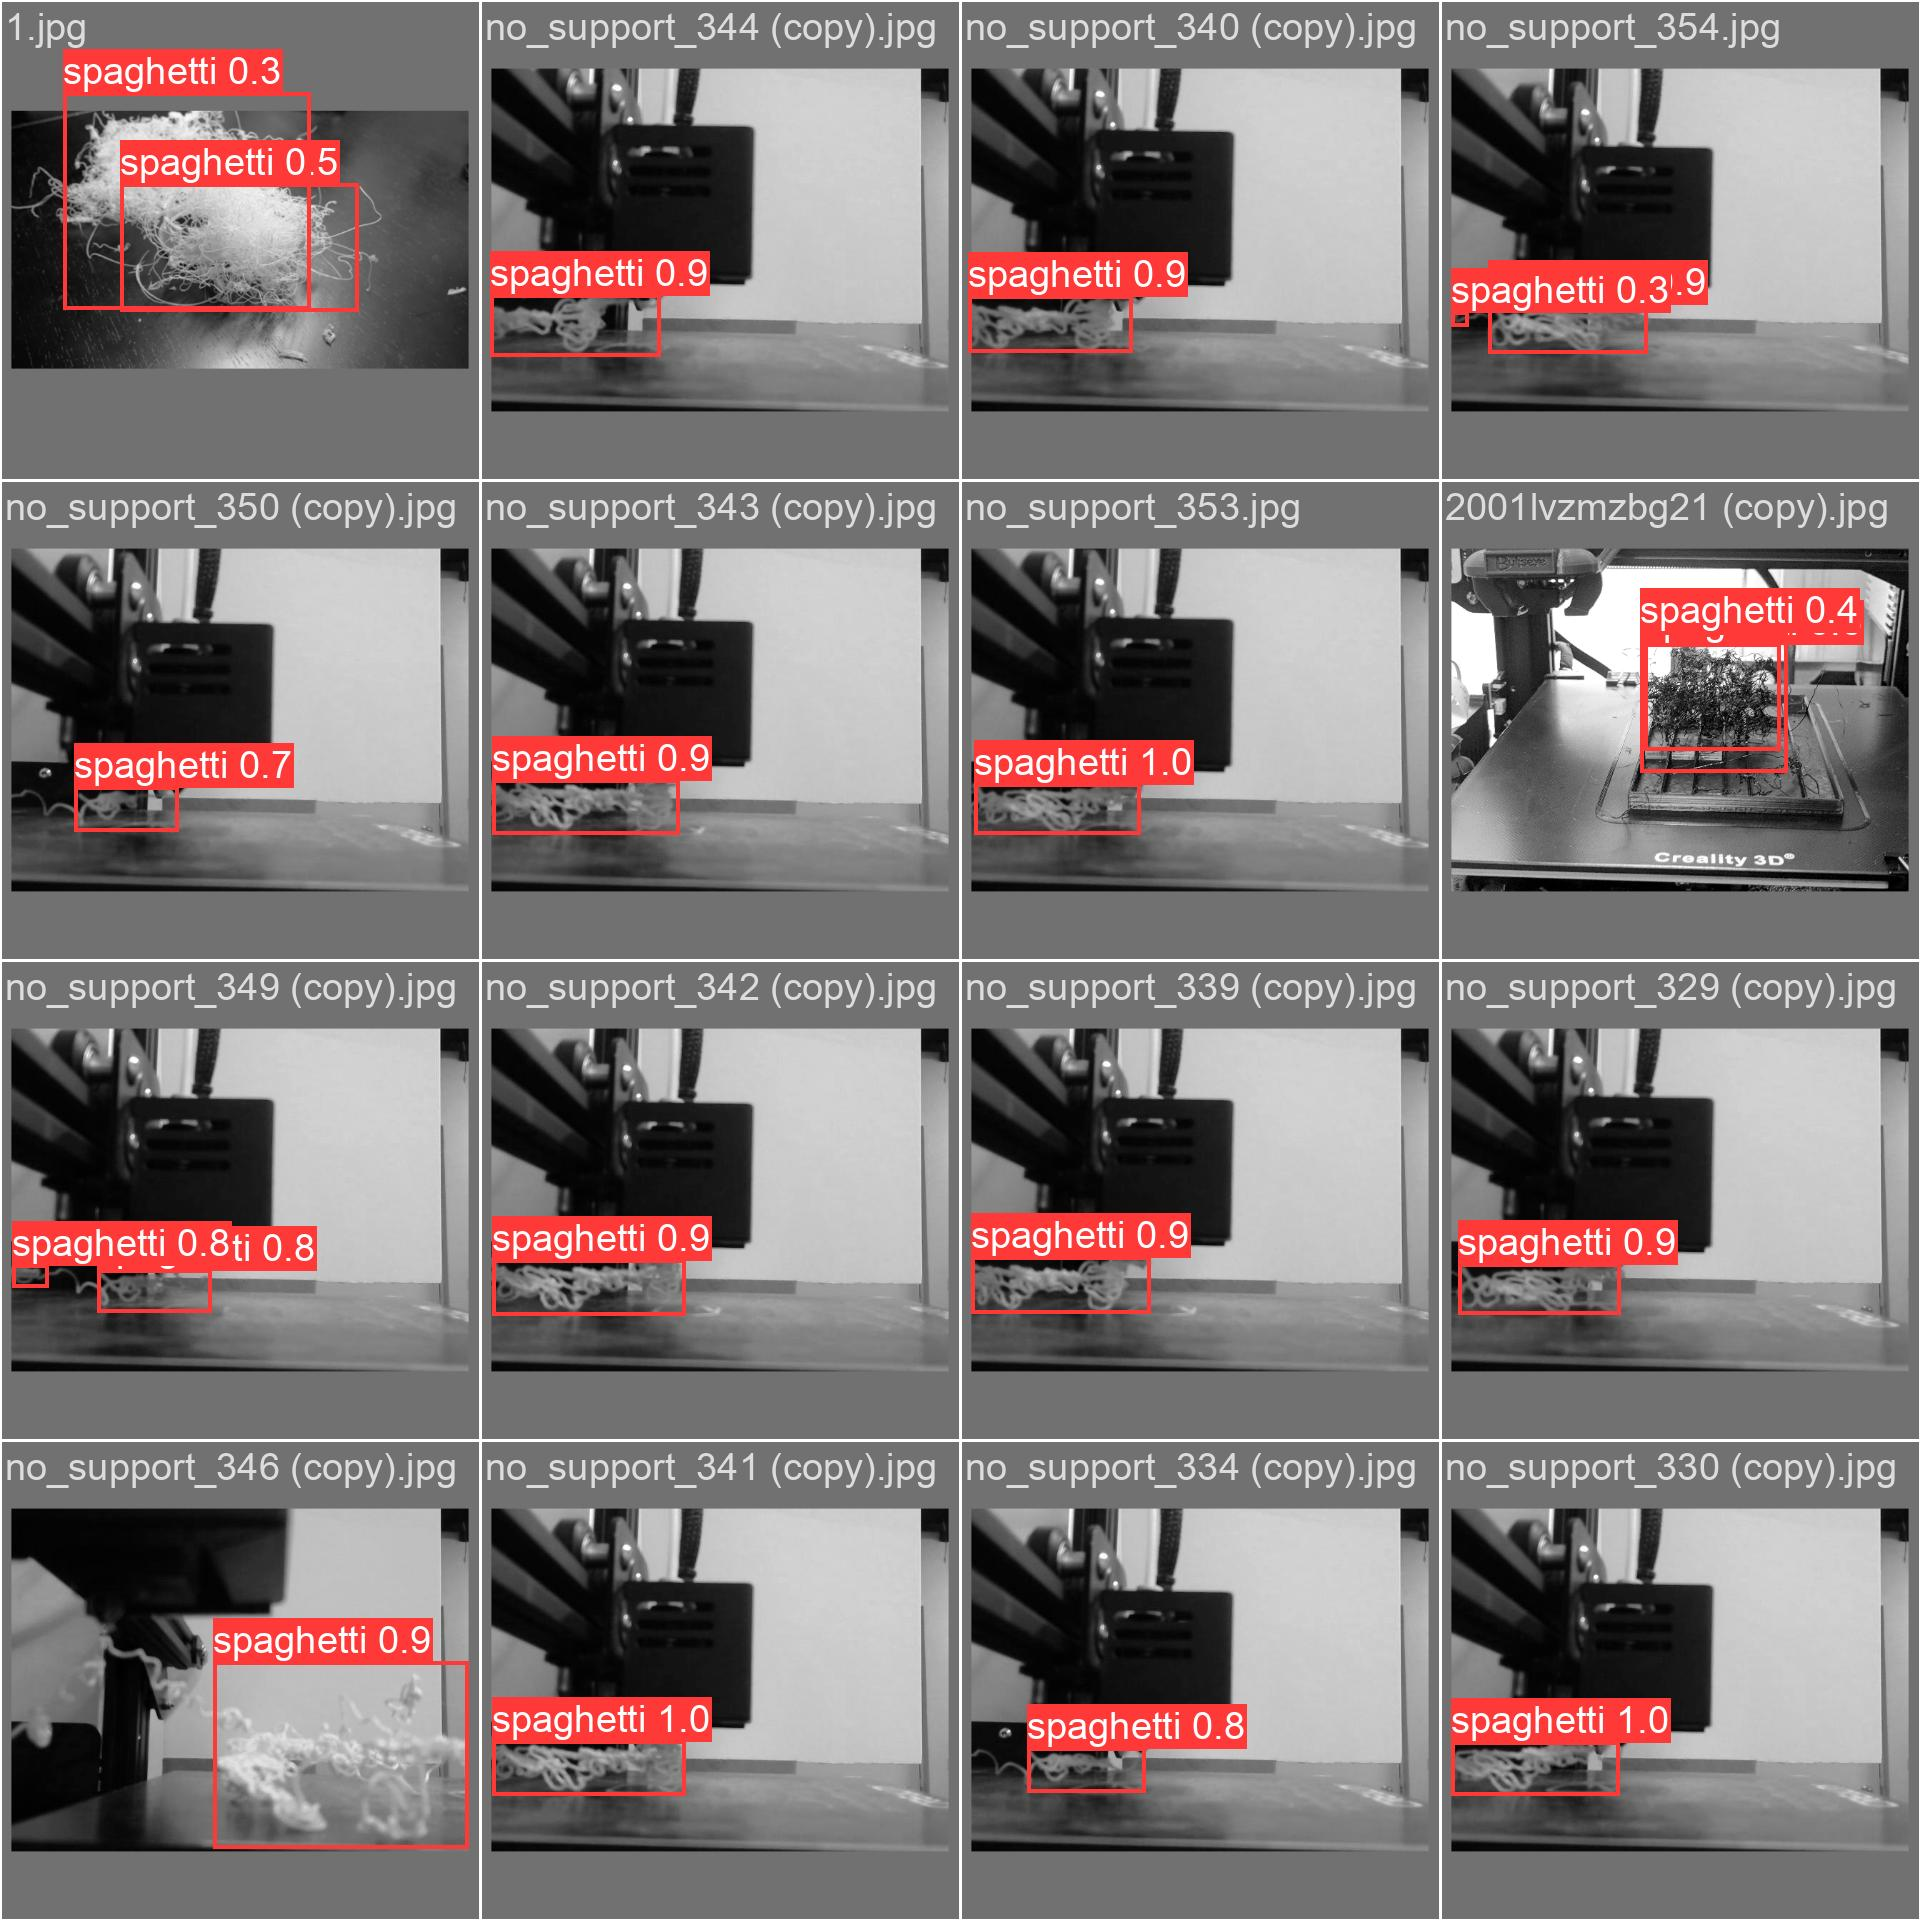
\includegraphics[width=1.2\linewidth]{val_batch0_pred.jpg}}
    \caption{Prediction of model on Images}
    \label{fig:grpahPrediction}
\end{figure}

\clearpage
\section{Conclusion}
The model's accuracy is currently satisfactory, but there is potential for improvement by incorporating additional data that includes real-life images.

\newpage
\clearpage
\begin{thebibliography}{9}

    \bibitem{onlineOpenSource1}
        Dataset: \href{https://www.kaggle.com/datasets/justin900429/3d-printer-defected-dataset}{3D-Printer Defected Dataset}: \\
        {\footnotesize \url{https://www.kaggle.com/datasets/justin900429/3d-printer-defected-dataset}}
    \bibitem{onlineOpenSource2}
        Dataset: \href{https://www.kaggle.com/datasets/mikulhe/3d-printing-errors}{3D printing errors}: \\
        {\footnotesize \url{https://www.kaggle.com/datasets/mikulhe/3d-printing-errors}}
    \bibitem{labelingTool1}
        Computer Vision Annotation Tool: \href{https://www.cvat.ai/}{CVAT}: \\
        {\footnotesize \url{https://www.cvat.ai/}}
    \bibitem{labelingTool2}
        Visual Object Tagging Tool: \href{https://github.com/microsoft/VoTT}{VoTT}: \\
        {\footnotesize \url{https://github.com/microsoft/VoTT}}
    \bibitem{labelingTool3}
        MakeSense: \href{https://www.makesense.ai/}{MakeSense}: \\
        {\footnotesize \url{https://www.makesense.ai/}}
    \bibitem{imagesOnlineTool}
    Resizepixel: \href{https://www.resizepixel.com}{Resizepixel}: \\
        {\footnotesize \url{https://www.resizepixel.com}}

    \end{thebibliography}

\end{document}
